\documentclass{article} % For LaTeX2e
\usepackage{iclr2017_conference,times}
\usepackage{hyperref}
\usepackage{url}
\usepackage{graphicx}

\title{GourmetNet}


\author{Metehan YILDIRIM \& Mete Han KAHRAMAN \& Ilayda CAVUSOGLU  \\
Department of Computer Engineering\\
Hacettepe University\\
Ankara, Turkey \\
}

% The \author macro works with any number of authors. There are two commands
% used to separate the names and addresses of multiple authors: \And and \AND.
%
% Using \And between authors leaves it to \LaTeX{} to determine where to break
% the lines. Using \AND forces a linebreak at that point. So, if \LaTeX{}
% puts 3 of 4 authors names on the first line, and the last on the second
% line, try using \AND instead of \And before the third author name.

\newcommand{\fix}{\marginpar{FIX}}
\newcommand{\new}{\marginpar{NEW}}

%\iclrfinalcopy % Uncomment for camera-ready version

\begin{document}


\maketitle

\begin{abstract}
In our report we explain the process of building a recommendation system for Yelp. Then focus the work we have done so far which is categorizing restaurants. We did this so later we can build a recommendation system on top of it. We first tried to use the restaurants of tags and using Word2Vec$^1$. Then getting word vectors we tried to apply K-Means Cluster$^2$ method to get some categories. This approach has failed and later we tried using manual categories.
\end{abstract}

\section{A Food Recommendation System : GourmetNet}

Our goal is to develop a food recommendation system for Yelp. The program will learn a person's taste according to the person's previous ranks that are given to restaurants and recommend a restaurant.\\

The research field for recommendation systems are not very active. Despite the interest of the companies on this topic. We found this topic  to be very practical for real life purposes.\\
 
\section{Related Work}

This is not a hot area on Machine Learning. But there is a lot of research caused by the industry on recommendation systems.$^3$ This topic comes up usually as Collaborative Filtering. We specifically looked at recommendation systems for Yelp.$^{4, 5, 6}$ \\

All approaches first worked on categorizing the foods because the data was sparse. Then using K-Nearest Neighbour and Collaborative Filtering on this categories. And most approaches also used a Graph we have yet to use it and we will see if it will be needed.


\section{Methodology}

There are many approaches to this but we preferred the baseline method the collaborative filtering. Collaborative filtering can be applied in two ways, a narrow one and a more general one. 


Narrow one is a method that makes automatic predictions. It collects preferences or taste information from many users. Then predicts about a user's interests. In our case narrow one will be used.



First problem is the sparseness of our data. Applying K-Nearest Neighbours$^7$ on this data is very impractical. So first we need to group our data. To do that Google's pretrained Word2Vec$^8$ corpus was going to be used. We thought using about them on the restaurant tags. After grouping our data with Word2Vec vectors K-Means Clustering was going to be applied. We later saw that this approach didn't work. For more information please seek section 4.


K-means clustering partitions N observations into k clusters. Each observation belongs to the cluster with the nearest mean. A observation is a prototype of it's own cluster. Objective function :
$$ J = \sum^{k}_{j=1}\sum^{n}_{i=1}\underbrace{\|x_{i}^{(j)}-c_{j}\|}_{distance}$$
$c_{j}$ : is the centre of the cluster\\
$x_{i}^{(j)}$ : is the data point\\

\section{Experimental Evaluation}

We are going to use Yelp dataset. Yelp data set includes many attributes. We analyse them and choose the most appropriate ones. 

The required business attributes are stars , review$\_$count, name, city, categories and business$\_$id. We shall recommend a restaurant  which belongs to the city that the user is currently located so city attribute is needed. Restaurants that do not have "categories" attribute is going to be deleted.

The required user attributes are average stars and user$\_$id.

For both users and cities average rate will be used.

We stripped the data only using these features. On some restaurants some fields were empty so we disregarded those. On closer observation we saw that majority of the shops weren't even restaurants. So we disregarded every shop without the tag named "Restaurant". And then we also disregarded restaurants with reviews less than 10. So after this we had around 25000 rows. \\

\subsection{Word2Vec on K-Means Approach}

So to categorize that we first thought of using Word2Vec for semantic similarities on tags and then using K-Means Clustering to group similar businesses together. This approach failed. Below you can see some examples of the clustering. We picked K as 100 and this is the result. As you can see "chinese" and "american" has the same label. This is not desired for us. So we needed a different approach.

\begin{center}
\begin{tabular}{ll}
\multicolumn{1}{c}{\bf Category}  &\multicolumn{1}{c}{\bf Label}
\\ \hline \\
Shopping	&	1 \\
Bar         &	5 \\
Nightclub	&  	5 \\
halal		& 11\\
japanese	& 24\\
american	& 34\\
chinese	& 34\\
italian	& 36\\
french	& 41\\
fries		& 72\\
sushi		& 72\\
club		& 76\\
turkish	& 76\\
coke		& 76\\
hamburger	&	78  \\
hotdog		&	78\\
cheeseburger &	 78\\
steak		& 78\\
pencil	& 94\\
potato	& 98\\

\end{tabular}
\end{center}
\newpage

\subsection{Manual Categorization}

So we analysed the data even further and observed that most restaurant categories had  their cuisine names. So we clustered our data on cuisines. We are thinking about clustering each cuisine clusters based on their other tags.


\begin{center}
  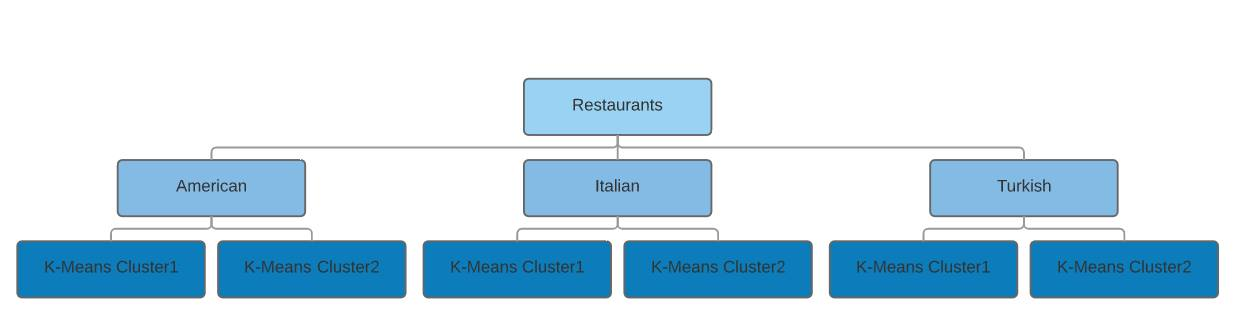
\includegraphics[width=\linewidth]{tablo.png}
\end{center}





\section{References}

[1] (\url{https://papers.nips.cc/paper/5021-distributed-representations-of-words\\-and-phrases-and-their-compositionality.pdf}) 

[2] (\url{https://msu.edu/~ashton/classes/866/papers/2010_jain_kmeans_50yrs__clustering_review.pdf}) 

[3] (\url{https://msu.edu/~ashton/classes/866/papers/2010_jain_kmeans_50yrs__clustering_review.pdf}) 


[4](\url{http://snap.stanford.edu/class/cs224w-2012/projects/cs224w-054-final.pdf})
 

[5](\url{https://pdfs.semanticscholar.org/8b2b/ada22181916196116f1711d456ea212f2b3b.pdf})



[6](\url{https://pdfs.semanticscholar.org/a7d2/5c03ec2a7dfe54c7b2e39729e906283e8e07.pdf})


[7](\url{https://msu.edu/~ashton/classes/866/papers/2010_jain_kmeans_50yrs__clustering_review.pdf}) 


[8](\url{http://www.gelbukh.com/ijcla/2014-1/IJCLA-2014-1-Complete.pdf#page=27})



\end{document}
